\documentclass{article}

\usepackage{lipsum}
\usepackage[margin=2cm, left=2cm, includefoot]{geometry}
\usepackage{graphicx}
\usepackage{float}
\usepackage{hyperref}

% Header and footer
\usepackage{fancyhdr}
\pagestyle{fancy}

\rhead{}
\lhead{}
\fancyfoot{}
\fancyfoot[R]{\thepage}
\renewcommand{\headrulewidth}{0pt}
\renewcommand{\footrulewidth}{0pt}
%

\begin{document}
	
	\begin{titlepage}
		\begin{center}
			\line(1,0){500}\\
			[6mm]
			\huge{\bfseries Software Requirements Specification}\\
			\line(1,0){500}\\
			[5mm]
			
\includegraphics[width=150px]{../images/AWorldOfPlants.png}
			\\
			[5mm]
			\large\textbf{Project:}\\A World of Things\\
			[3mm]
			\large\textbf{Client:}\\Julian Hambleton-Jones\\
			[3mm]
			\large \textbf{Team:}\\Funge\\
			\line(1,0){500}\\
			[5mm]
			\large \textbf{Team Members:}\\
			[3mm]
			\large 14214742 - Matthew Botha\\
			\large 14446619 - Gian Paolo Buffo\\
			\large 14027021 - Matthias Harvey\\
			\large 14035538 - Dillon Heins\\[3mm]
		\end{center}
	\end{titlepage}
	
	\cleardoublepage
	\thispagestyle{empty}
	\tableofcontents
	\cleardoublepage
	\setcounter{page}{1}

\section{Use Cases}
	\subsection{User Management Subsystem}
		\begin{figure}[H]
			\centering
			\includegraphics[width=\textwidth]{../images/user-management-subsystem.png}
			\caption{The \emph{User Management} subsystem}
		\end{figure}
		\subsubsection{Register Account}
			A user should be able to register an account using the \emph{Register Account} page. The user should not be able to log in before they have registered. Once the user has registered an account, they should be able to \emph{Log In (1.2)}.
		\subsubsection{Log In}
			Once a user has been registered, the user should be able to log into their account. They cannot log in before registering. They have to provide the correct username and password in order to log in. Once the correct credentials have been given, they are taken to the \emph{Home Page} where they can \emph{Edit Details (1.3)}, \emph{View Gamification Information (1.4)} and access the \emph{Plant/Device Management Subsystem (2)}.
		\subsubsection{Edit Details}
			Once a user has logged in, they can edit their details from the \emph{Edit Details} page. They can change their email, password and other personal details, but cannot change their username. They can then save the changes and they will take effect immediately.
		\subsubsection{View Gamifaction Information}
			Once a user has logged in, they can view their current gamification information. This will show them their standings in the leaderboards, the awards and badges they have achieved and progress to following markers.
	
	\newpage
	\subsection{Plant/Device Management Subsystem}
		\begin{figure}[H]
			\centering
			\includegraphics[width=\textwidth]{../images/plant-management-subsystem.png}
			\caption{The \emph{Plant Management} subsystem}
		\end{figure}
		\subsubsection{Create Plant}
			The user should be able to create a plant on their account. Through this, they can add the device the plant is connected to, add the type of plant, select which sensors are connected to the plant etc.
		\subsubsection{View Plant Status}
			The user should be able to view the status of their existing plants. This page will show the most recent data collected by the device as well as historical data for a specific plant. The date of the data is dislpayed and the user has the option of requesting a forced update from the device.
		\subsubsection{Edit Plant Details}
			The user should be able to edit the details of an existing plant. They can change the basic information (type of plant etc) as well as \emph{Add Sensor to Device (2.4)}, \emph{Remove Sensor from Device (2.5)} and \emph{Edit Plant Configuration/Settings (2.6)}.
		\subsubsection{Add Sensor to Device}
			The user should be able to select a device and add a sensor to the device.
		\subsubsection{Remove Sensor from Device}
			The user should be able to select a device and remove a sensor from the device. The removed sensor should not be removed from the historical view, but will not be shown on the \emph{View Plant Status (2.2)} and the \emph{Edit Plant Configuration/Settings (2.6)} pages.
		\subsubsection{Edit Plant Configuration/Settings}
			The user should be able to select a plant and edit the current configuration for the configurable settings on the device. This includes water cycles, light settings, air flow etc.
		\subsubsection{Remove Plant}
			The user should be able to remove a plant. This will disable the connected device and disable the \emph{View Plant Status (2.2)} and the \emph{Edit Plant Configuration/Settings (2.6)} pages for that plant, but the plant should still be in the historical view.
	
	\newpage
	\subsection{Device Communications Subsystem}
		\begin{figure}[H]
			\centering
			\includegraphics[width=\textwidth]{../images/device-communications-subsystem.png}
			\caption{The \emph{Device Communications Subsystem} subsystem}
		\end{figure}
		\subsubsection{Send Updated Settings/Configuration to Device}
			The Lambda server should be able to send settings set in the \emph{Edit Plant Configuration/Settings (2.6)} page and send them to the device. This is done by updating the device shadow and synchronising the device with its shadow.
		\subsubsection{Send Readings Summary to Lambda}
			On a regular schedule, the device should send its summary of readings from the sensors to the Lambda server. The subscribed users can then view the summary in the \emph{View Plant Status (2.2)} page and historical summary.

\section{Services Contracts}
	\subsection{Register}
		\begin{figure}[H]
			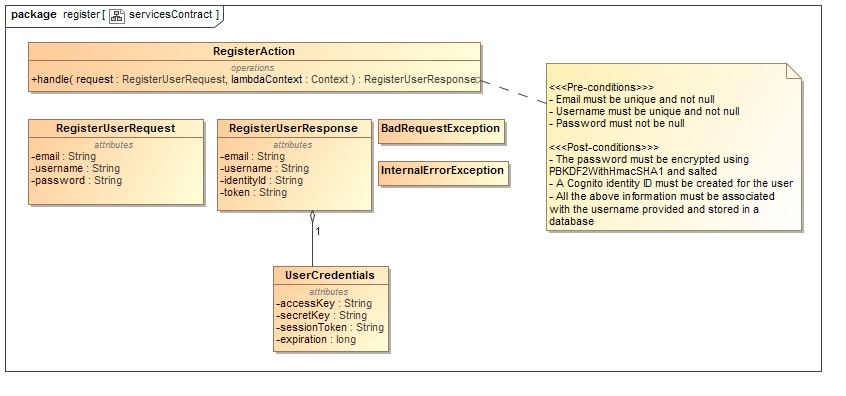
\includegraphics[width=\linewidth]{../images/ServicesContracts/register.jpg}
			\caption{Services Contract - Register User}
		\end{figure}
		
	\subsection{Login}
		\begin{figure}[H]
			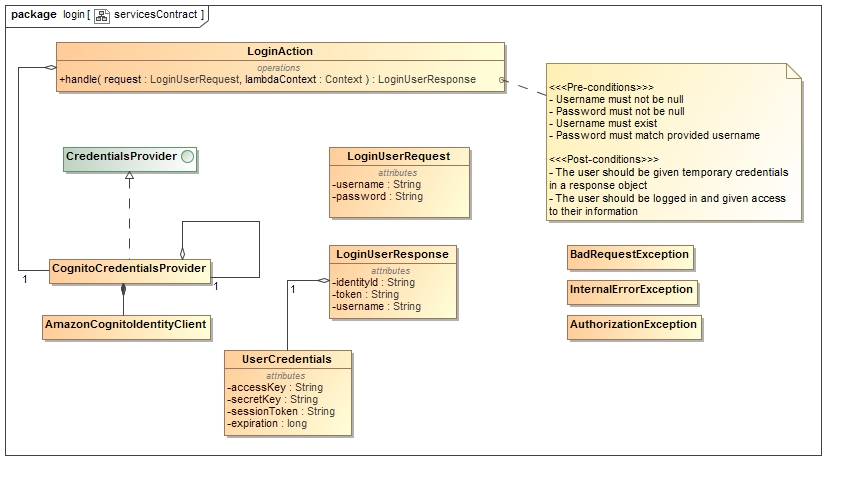
\includegraphics[width=\linewidth]{../images/ServicesContracts/login.jpg}
			\caption{Services Contract - Login User}
		\end{figure}
	
	\subsection{Create Plant}
		\begin{figure}[H]
			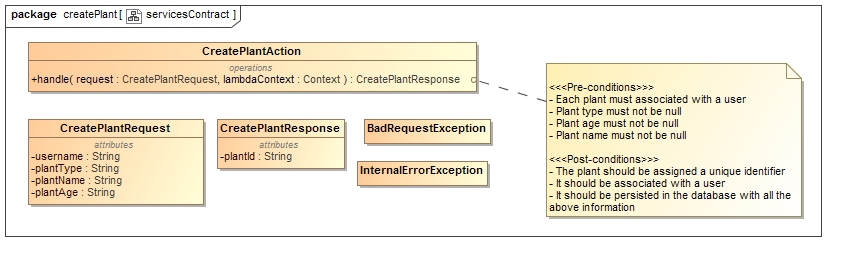
\includegraphics[width=\linewidth]{../images/ServicesContracts/createPlant.jpg}
			\caption{Services Contract - Create Plant}
		\end{figure}
		
	\subsection{List User Plants}
		\begin{figure}[H]
			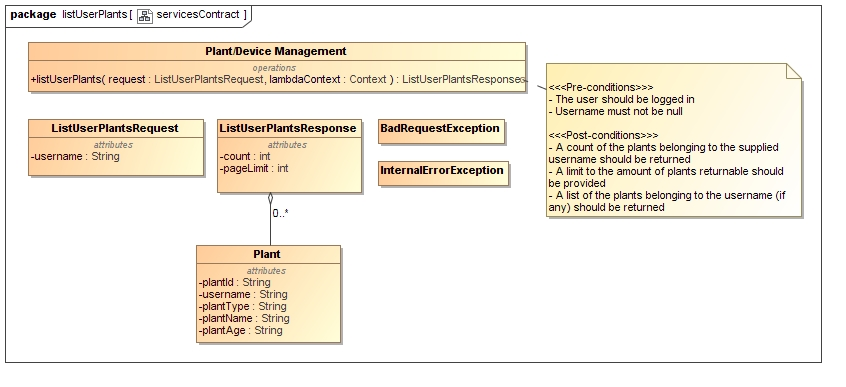
\includegraphics[width=\linewidth]{../images/ServicesContracts/listUserPlants.jpg}
			\caption{Services Contract - List User Plants}
		\end{figure}
		
	\subsection{Update Plant}
		\begin{figure}[H]
			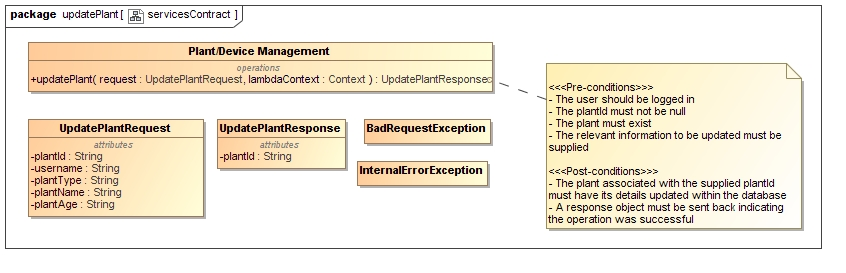
\includegraphics[width=\linewidth]{../images/ServicesContracts/updatePlant.jpg}
			\caption{Services Contract - Update Plant}
		\end{figure}
		
	\subsection{Delete Plant}
		\begin{figure}[H]
			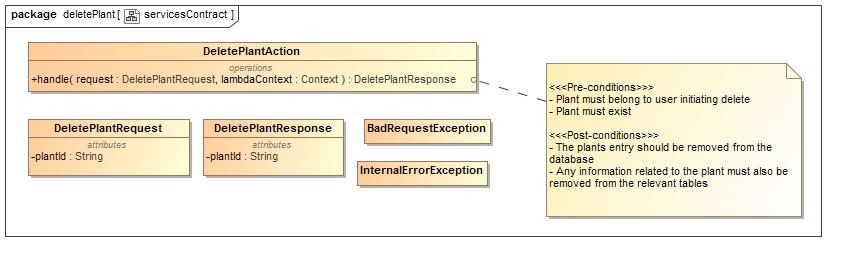
\includegraphics[width=\linewidth]{../images/ServicesContracts/deletePlant.jpg}
			\caption{Services Contract - Delete Plant}
		\end{figure}
\end{document}